\section{Okrogla cev}

V tej nalogi sem  računal pretok po cevi z metodo končnih elementov (MKE). Pri tem računsko domeno razdelim na podobmočja imenovana končni elementi (KE), kjer aproksimiram neznano funkcijo s polinomi in vozliščnimi vrednostmi 
\begin{equation}
    v(x,y) = \sum_i^{N_e}\;V_i\,\psi_i(x,y).
\end{equation}
Diferencialna enačba za pretok viskozne tekočine
\begin{equation}
    \nabla^2 v(x,y) = C = konst.
\end{equation}
se zaradi množenja z utežno funkcijo $w(x,y)$ in integracije per-partes po območju KE, označenim z $\omega$ prevede na šibko integralsko obliko
\begin{equation}
    \nabla v(x,y)\,\nabla w(x,y) \Biggr |_{\Gamma} - \int_{\omega}\,\nabla v(x,y)\, \nabla w(x,y) d\omega = C\, \int_{\omega}\,w\,d\omega,
\end{equation}
kjer je odvod nad $v(x,y)$ le prvega reda. Robni pogoj za sekundarno spremenljivko (toplotni tok) je v tem primeru eksaktno izpoljen, saj je odvod na meju območja $\Gamma$ zajet v DE, vendar v tem primeru Neumanovega RP sploh ni! Uporabim Galerkinov pristop in izberem utežne funkcije $w$ enake oblikovnim $\psi$.

Ker sem mrežil s trikotnimi KE, so oblikovne funkcije polinomi prvega reda in se integrali poenostavio do te mere, da je mogoč njih analitičen izračun s pomočjo katerega dobimo sistem enačb za KE
\begin{equation}\label{eqn:KE}
    \mathbf{K}\cdot\mathbf{v}= C\;\frac{A_i}{3}\,
    \begin{Bmatrix}
        1\\ 1\\ 1
    \end{Bmatrix},
\end{equation}
kjer je $\mathbf{v}=(V_i,V_j,V_k)$ vektor vozliščnih vrednosti (neznak), $A_i$ površina KE, $\mathbf{K}$ pa togostna matrika KE
\begin{equation}
    \mathbf{K} = \begin{bmatrix}
            \begin{aligned}
                (x_2 - x_3)^2 +\\ + (y_2 - y_3)^2
            \end{aligned} &
            \begin{aligned}
                - [(x_1 - x_3)(x_2 - x_3) +\\+ (y_1 - y_3)(y_2 - y_3)]
            \end{aligned} &
            \begin{aligned}
                (x_1 - x_2)(x_2 - x_3) +\\+ (y_1 - y_2)(y_2 - y_3)
            \end{aligned} \\ \\

            \begin{aligned}
                - [(x_1 - x_3)(x_2 - x_3) +\\+ (y_1 - y_3)(y_2 - y_3)]
            \end{aligned} &
            \begin{aligned}
                (x_1 - x_3)^2 +\\+ (y_1 - y_3)^2
            \end{aligned} &
            \begin{aligned}
                - [(x_1 - x_2)(x_1 - x_3) +\\+ (y_1 - y_2)(y_1 - y_3)]
            \end{aligned} \\ \\

            \begin{aligned}
                (x_1 - x_2)(x_2 - x_3) +\\+ (y_1 - y_2)(y_2 - y_3)
            \end{aligned} &
            \begin{aligned}
                - [(x_1 - x_2)(x_1 - x_3) +\\+ (y_1 - y_2)(y_1 - y_3)]
            \end{aligned} &
            \begin{aligned}
                (x_1 - x_2)^2 +\\+ (y_1 - y_2)^2
            \end{aligned} \\  
        \end{bmatrix}.
\end{equation}

Izraz za en KE nato razširim na vse prostostne stopnje in za vsak KE prištejem vrednosti po enačbi \ref{eqn:KE}. Dobljeni globalni sistem enačb $\mathbf{K}_{gl} \cdot \mathbf{v}_{gl} = \mathbf{c}_{gl}$ je pasoven, kjer širino pasu določa največja razlika med indeksoma vozlišč v KE in se lahko reši s poljubnim algoritmom, desna stran $\mathbf{c}_{gl}$ pa zajema tudi robne pogoje.

Zanje sem predpostavil nezdrsne robne pogoje in postavil $v=0$ na vsakem vozlišču na obodu cevi.

Prvo sem preizkusil delovanje na najenostavnejšem primeru cevi okroglega preseka, ki sem jo naivno generiral vozlišča v cilindričnem koordinatnem sistemu in nato nanje napel Delaunay-evo triangulacijo iz \texttt{scipy.spatial.Delaunay}. Taka mreža sicer ni idealna, saj so KE v središču zelo stisnjeni in zgoščeni, skupaj z izračunanimi vozliščnimi vrednostmi pa je mreža prikazana na spodnji levi sliki, za večje število vozlišč pa je tak prikaz nepregleden, so na desni strani prikazane izolinije preko aproksimacije fukcije $v(x,y)$ po KE.

\begin{figure}[ht]
    \centering
    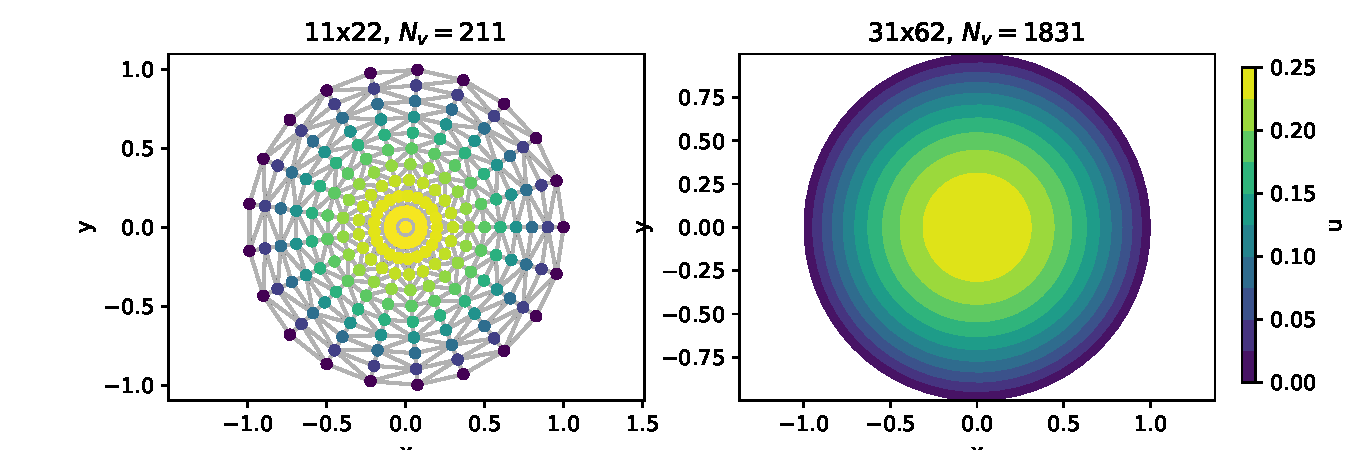
\includegraphics[width=\linewidth]{7.nal_slike/krog_mreza.pdf}
    \caption{Rezultat hitrostnega polja v okrogli cevi}
\end{figure}

Za izračun pretoka moramo razrešiti integral $\dot V = \int\,v(x,y)\,dA$, kjer upoštevamo uporabljeno aproksimacijo za $v(x,y)$, zato se integral prevede na vsoto po KE
\begin{equation}
    \dot V = \sum_{i}^{N_{el}}\, \sum_{j}^{N_v=3}\, V_j\, \frac{A_i}{3} = \sum_{i}^{N_{el}}\, \frac{A_i}{3}\, (V_i+V_j+V_k)
\end{equation}
kjer so $V_i,V_j,V_k$ izračunane vozliščne vrednosti za tovozliščni KE.

Na spodnji sliki je prikazan Poiuseuillov koeficient
\begin{equation}
    C = \frac{\dot V\, 8\,\pi\, \eta}{A^2\,dp},
\end{equation}
v brezdimenzijski obliki ($A=\eta=dp=1$), ki pričakujemo, da je za krog $C=1$. Le-ta popisuje lastnost cevi in z njegovo pomočjo lahko za vsako cev pri danih obratovalnih pogojih določimo pretok brez potrebe po izračunu integrala hitrostnega polja.

V dokumentu \footnote[1]{Duke University, Math 563 Lecture Notes: Differentiation, Richardson Extrapolation, pomlad 202, dostopno na \href{https://services.math.duke.edu/~jtwong/math563-2020/lectures/Lec2-derivatives.pdf}{povezavi}} je definirana Richardsonova ekstrapolacija
\begin{equation}\label{eq:richardson_1}
    A_k(h) = \frac{1}{4^k-1} \, \left(4^k\,A_{k-1}\left(\frac{h}{2}\right) - A_{k-1}\left(h\right)\right),
\end{equation}
ki za skalarni veličini $A(\frac{h}{2})$ in $A(h)$ izračuna nov približek. Pri tem je $k$ število vseh izračunov na prostorskih diskretizacijah v razmerju 2, zato lahko na tak način iterativno izboljšamo rezultat na red $O(h^{2\,k})$. Tako sem generirano mrežo zgoščeval za faktor 2 in na koncu izračunal ekstrapolirano vrednost k kateri konvergirajo izračuni. Ugotovil sem, da je to vrednost skoraj enaka pričakovani!

\begin{figure}[ht]
    \centering
    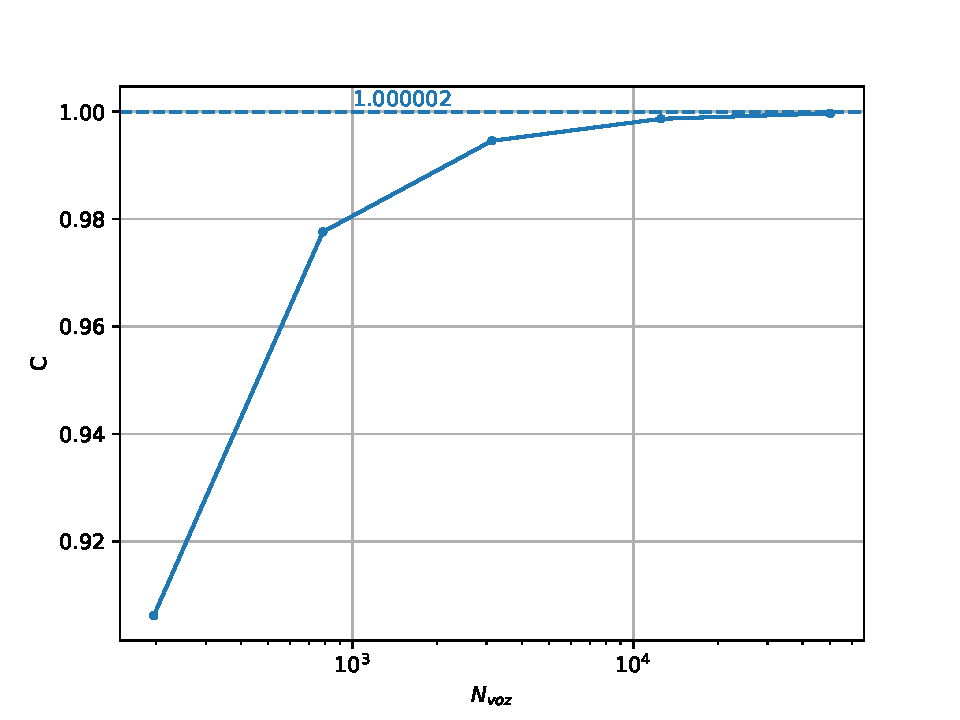
\includegraphics[width=0.7\linewidth]{7.nal_slike/konv_C_richardson_krog.pdf}
    \caption{Poiuseuillov koeficient za krog}
\end{figure}

\section{Polkrožna cev}

Tokovne razmere se bistveno spremenijo, ako cev ni popolnoma polna, temveč le do polovice. V tem primeru sem na gladini vode predpostavil robni pogoj $v=0$ in pričakujem zmanjšanje Poiuseuillovega koeficienta.

\subsection{Lastno mreženje}

Mrežo sem generiral na enak način kot za polno cev, ampak le do 180$^\circ$ in je prikazana na spodnji sliki, prav tako pa tudi prikaz izolinij aproksimacije hitrostnega polja za večje število vozlišč. Opazimo, da se največja hitrost zmanjša iz okoli 0,25 za krog na 0,10 za polkrog, prav tako pa se lega največje hitrosti premakne navzdol. Izgleda, kot da je v težišču cevi.

\begin{figure}[ht]
    \centering
    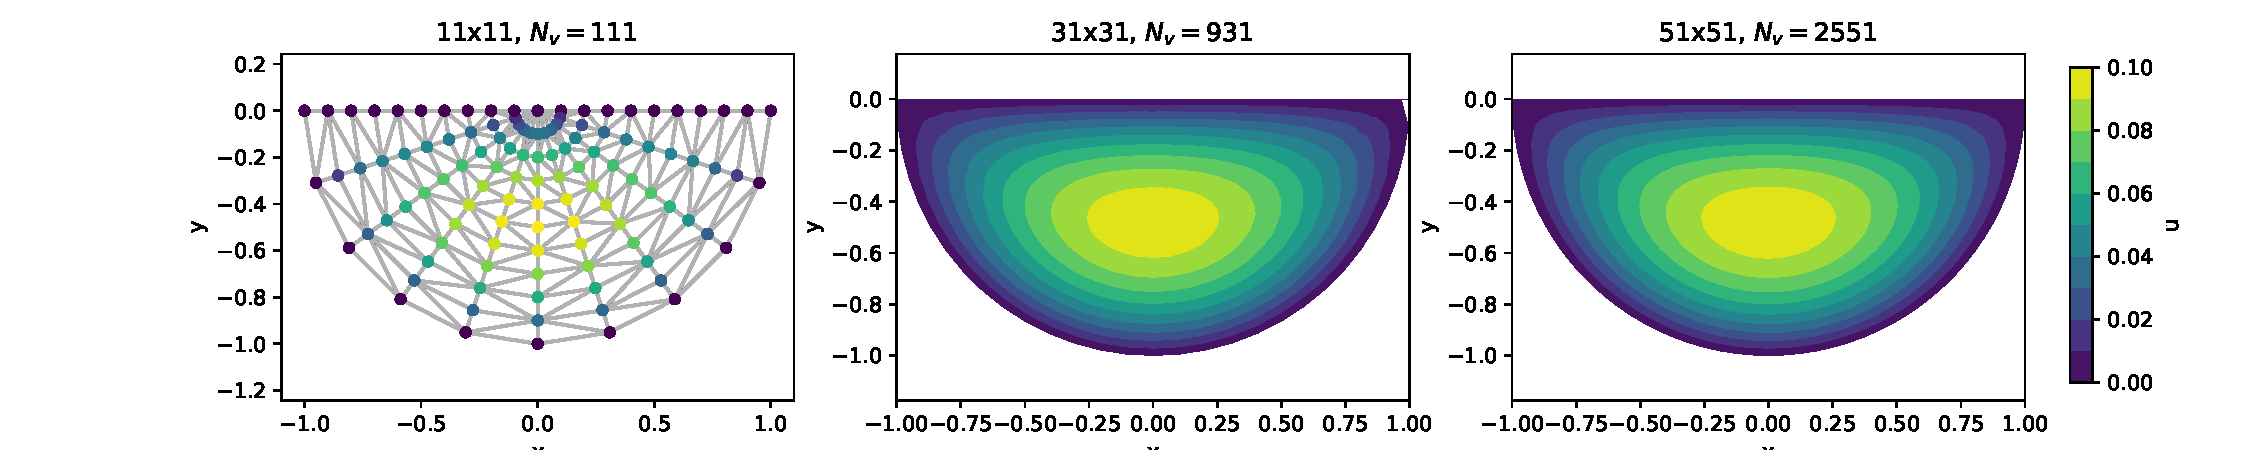
\includegraphics[width=\linewidth]{7.nal_slike/lastna_u.pdf}
    \caption{rezultati lastnega mreženja}
\end{figure}

\subsection{Komercialni programi}

Uporabil sem programa \textit{Ansys Student 2024 R1} in \textit{Abaqus Student 2021} za izdelavo mreže KE na polkrogu. Opazil sem, da je vsa čarovnija v generiranju točk, na katere se potem napne Delaunay-eva triangulacija, kar je razvidno iz spodnjih slik. Očitno so vozlišča drugače razporejena, čeprav je njih število enako. Tudi rezultati so primerljivi.

\begin{figure}[H]
    \centering
    \begin{subfigure}{\textwidth}
        \centering
        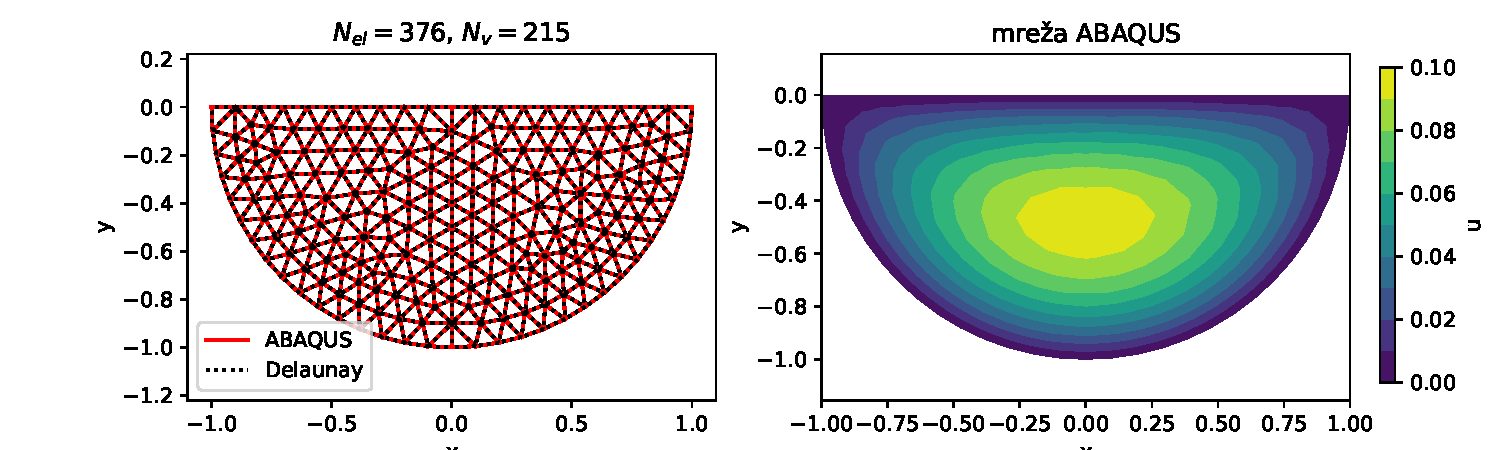
\includegraphics[width=\linewidth]{7.nal_slike/abaqus_rez.pdf}
        \caption{Abaqus}
    \end{subfigure}
    \begin{subfigure}{\textwidth}
        \centering
        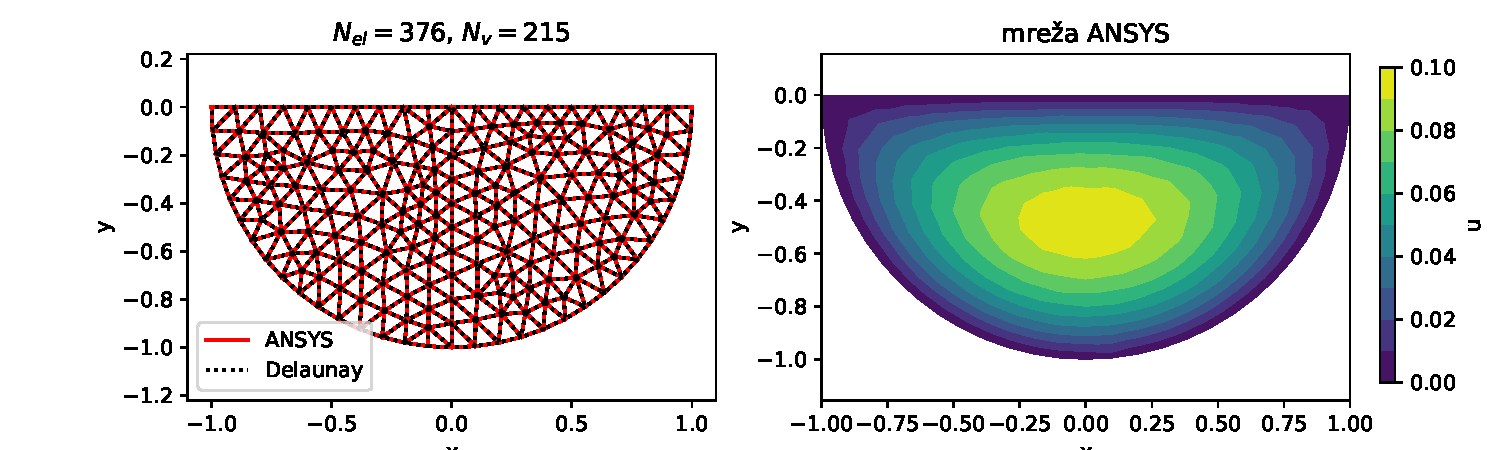
\includegraphics[width=\linewidth]{7.nal_slike/ansys_rez.pdf}
        \caption{Ansys}
    \end{subfigure}
    \caption{Mreža in rezultati komercialnih programov}
\end{figure}

\subsection{Primerjava med mrežami KE}

Čeprav je bilo polje aproksimacije hitrosti v vseh primerih podobno na oko, je razlika očitna pri Poiuseuillov-em koeficientu. Sedaj se tudi vidi kakovost mreže, saj sta oni iz komercialnih programov bližje pravi rešitvi že pri manj gosti mreži.

Ponovno sem izračunal ekstrapolirano vrednost, ki se za različne mreže razlikuje za red velikosti $10^{-6}$, velja pa poudariti, da mreže iz komercialnih programov niso bile zgoščevane točno za faktor 2. Koeficient je pričakovano manjši od onega za krog, vendar vseeno ni 1/2. Očitno zveza med površino preseka cevi in Poiuseuillovem koeficientu ni linearna!

\begin{figure}[ht]
    \centering
    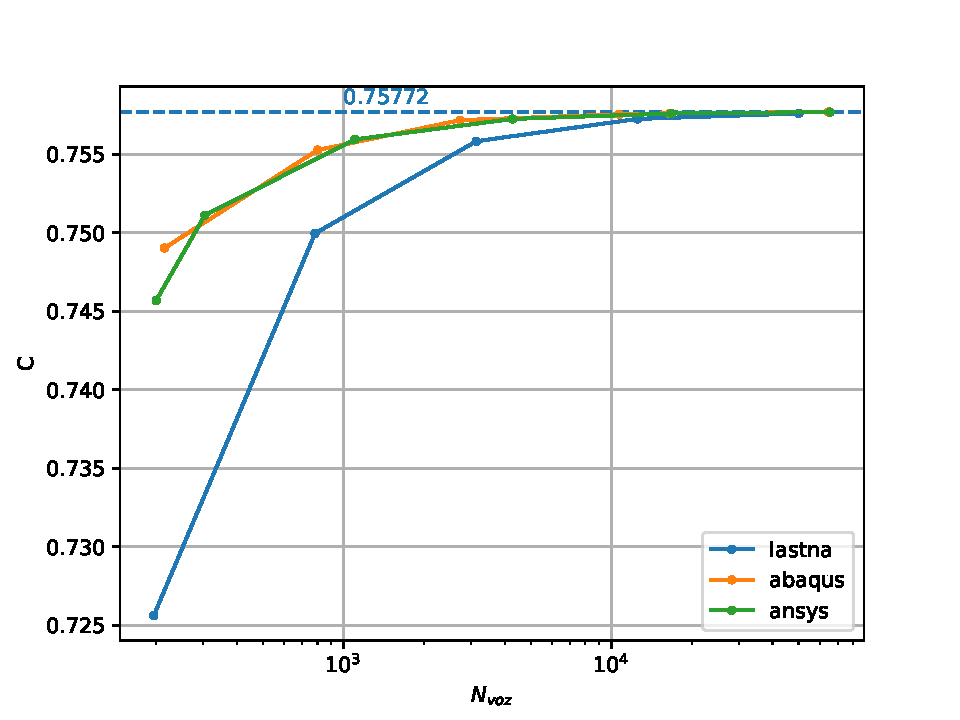
\includegraphics[width=0.71\linewidth]{7.nal_slike/konv_C_richardson_polkrog.pdf}
    \caption{Poiuseuillov koeficient za polkrožno cev}
\end{figure}

Prav tako lahko opazim, da se največja hitrost nahaja na ordinatni osi $x=0$, zato sem mreže generiral tako, da je mogoč prerez preko ordinate. Pri tem opazimo, kako je lahko sicer enako gosta mreža iz komercialnih programov bolj kakovostna od lastne. Pri ekstrapolaciji je ponovno razlika za $10^{-6}$, vendar je rezultat pri Abaqus-u še bolj vprašljiv zaradi čudnega poteka konvergence.

\begin{figure}[ht]
    \centering
    \begin{subfigure}{0.49\textwidth}
        \centering
        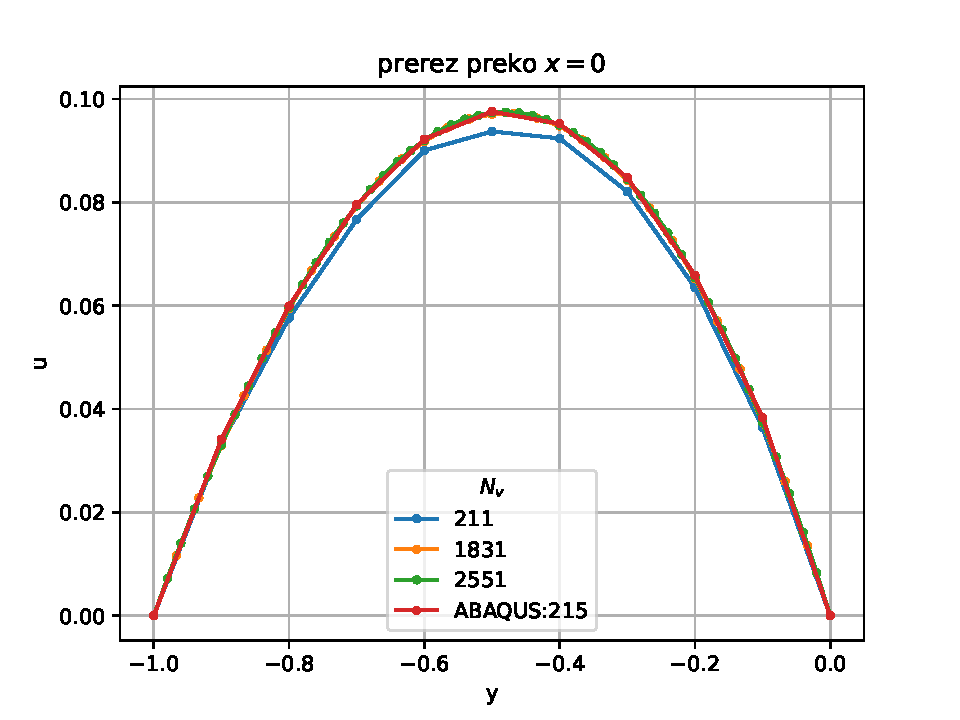
\includegraphics[width=\linewidth]{7.nal_slike/presek_polkrog.pdf}
        \caption{Hitrostni profil}
    \end{subfigure}
    \begin{subfigure}{0.49\textwidth}
        \centering
        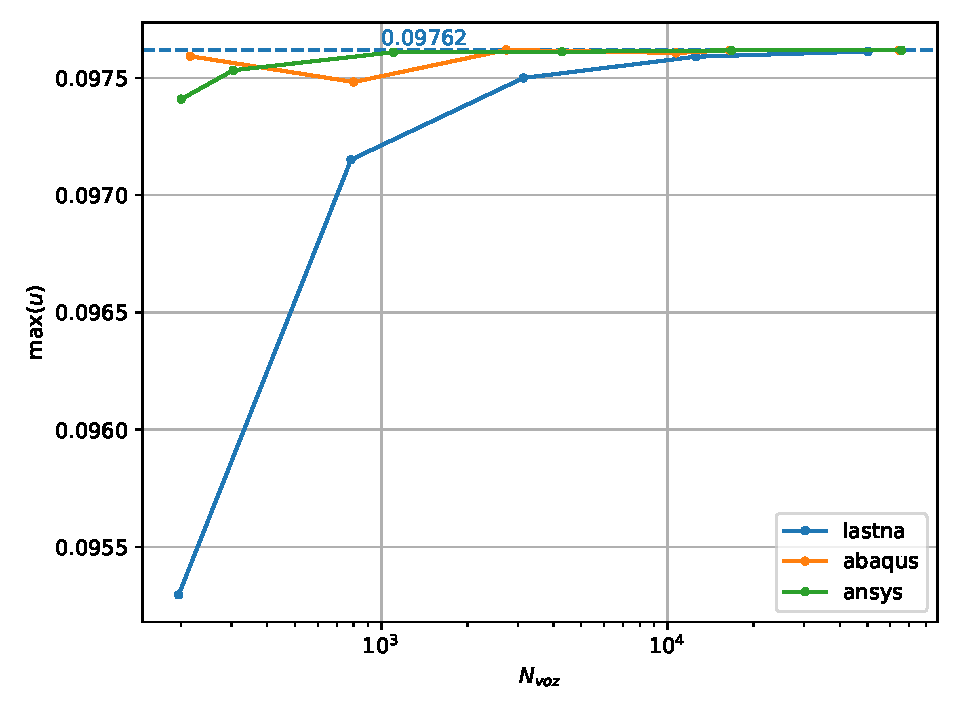
\includegraphics[width=\linewidth]{7.nal_slike/konv_max_u.pdf}
        \caption{Največja vrednost}
    \end{subfigure}
    \caption{Navpični presek preko sredine ($x=0$)}
\end{figure}

\section{Cev iz 5. naloge}

Sedaj obravnavam še presek cevi, kot je bil podan v 5. nalogi, po MKE. Mrežo sem generiral s programom Ansys, ki pa se tokrat ne ujema s triangulacijo Delaunay v Pythonu na enakih vozliščih. Zato je prikaz z izolinijami popačen, saj funkcija \\ \texttt{matplotlib.pyplot.tricontourf} uporablja Delaunay triangulacijo. Zato so na levi prikazne tudi vozliščne vrednosti z mrežo KE.

\begin{figure}[ht]
    \centering
    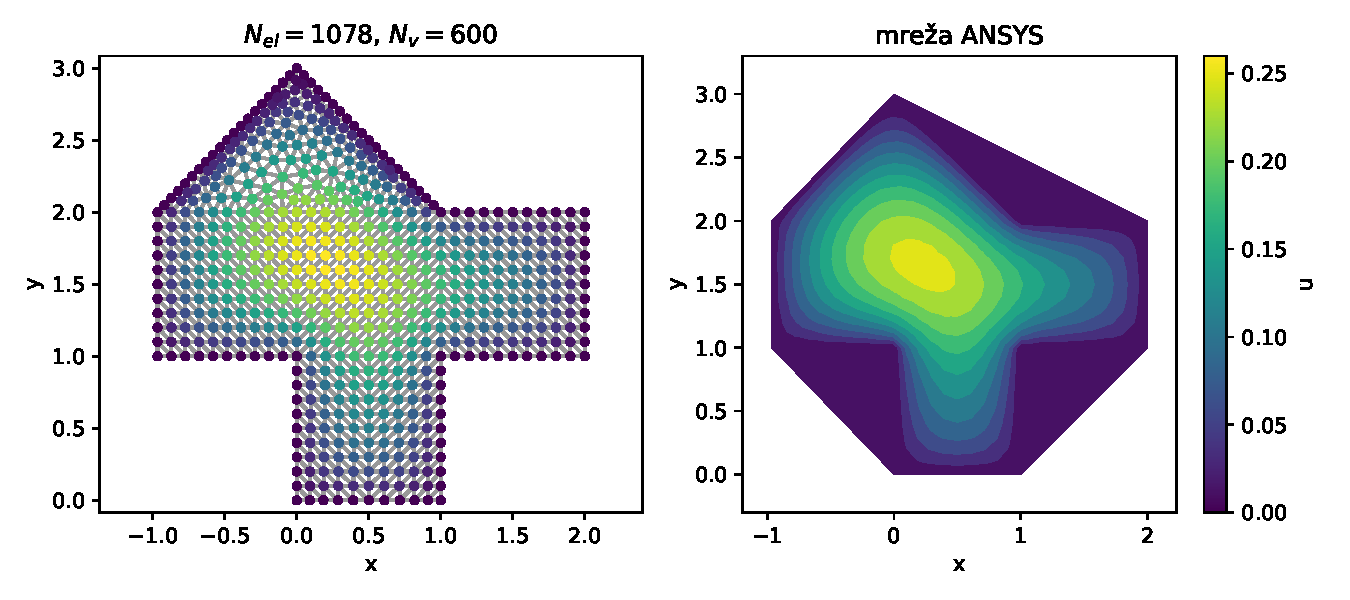
\includegraphics[width=\linewidth]{7.nal_slike/cev_nal2.pdf}
    \caption{Rezultati hitrostnega polja po MKE}
\end{figure}

Poiuseuillov koeficient je v tem primeru še manjši od polkrožne cevi, čeravno je površina preseka cevi večja od polkroga!

\begin{figure}[H]
    \centering
    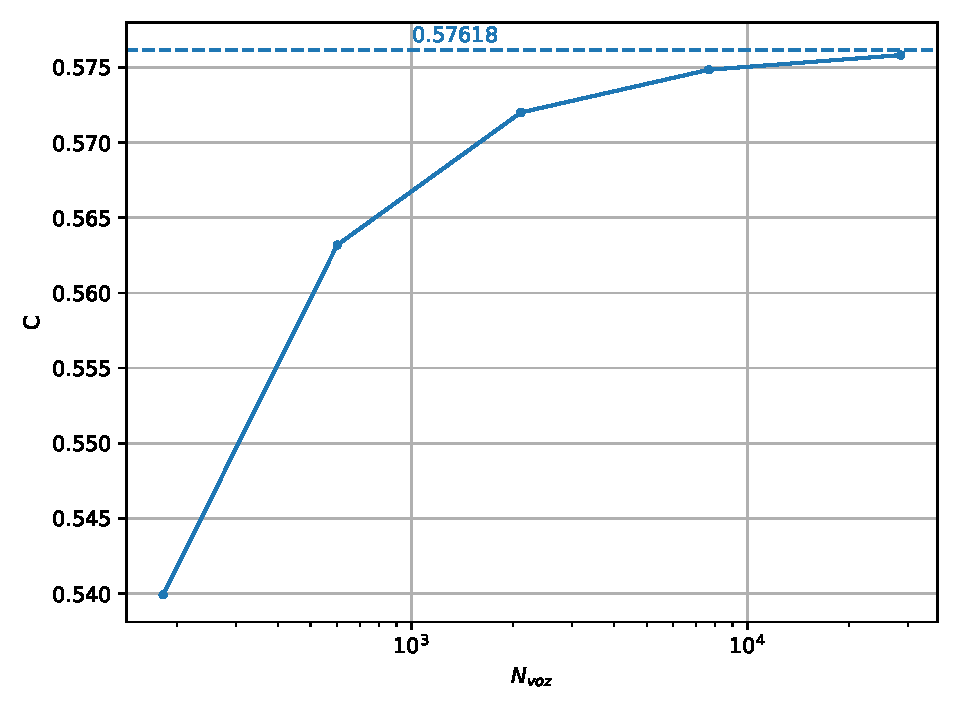
\includegraphics[width=0.7\linewidth]{7.nal_slike/konv_C_richardson_cev.pdf}
    \caption{Konvergenca Poiuseuillov-ega koeficienta}
\end{figure}

\noindent Sledi še primerjava z metodo končnih razlik (MKR) in MKE:

Pri obeh metodah so robni pogoji za primarno spremenljivko (hitrost) zajeti eksaktno, sekundarna (odvod primarne, pospešek) pa je eksaktno izpoljena pri MKE, pri MKR pa ne, ampak se aproksimira po Taylorjevi vrsti.

Pri MKE dobimo simetričen in pasoven sistem enačb, katerega širina je odvisna od kakovosti mreže, pri MKR pa za lepe geometrije in prostorske diskretizacije v 1D tri-, v 2D pet- in v 3D sedem-diagonalen sistem enačb. Oba lahko rešujemo na več načinov, v splošnem je za majhne sisteme hitreje, če jih rešujemo direktno, za velike pa iterativno. Ker lahko za Dirichletove robne pogoje, kjer je predpisana vrednost nič, preprosto izbrišemo enačbo iz sistema, je verjetno hitreje reševati sisteme, dobljene po MKE metodi, saj lahko izkoristimo značilno diagonalno obliko pri direktnem reševanju, dočim je za one po MKE bolj primeren katerikoli algoritem za redke matrike ali iterativen pristop.

Res pa je, da je lažje generirati mrežo za MKE in aplicirati robne pogoje, kot je to pri MKR.

\vspace{5mm}
Na spodnji sliki je prikazana časovna zahtevnost izračuna po MKE in MKR, kjer sem za reševanje po MKR uporabil metodo SOR, pri MKE pa direktno metodo z LU razcepom in delnim pivotiranjem za prva dva izračuna in sparse solver iz \texttt{scipy} za zadnja dva. Iteracije SOR sem prekinil, ko se Poiuseuillov koeficient ni spremenil za več kot $10^{-9}$, verjetno pa bi bilo bolj smiselno spremljati normo hitrostnega polja, saj se je koeficient ustalil precej hitro. Opazno naraste potreba po računskem času za večje sisteme, očitnejših časovnih razlik med metodama pa ni.

Predvsem je razlika z komercialnimi programi za MKE, kjer se sicer uporablja hitrejši programski jezik (C) in paralelizacija. V Abaqusu sem izračunal problem na enem jedru, v Ansysu pa na štirih. Programa sta uporabljala `sparse direct solver', očitne pohitritve zaradi paralelizacije verjetno zaradi majhnega sistema ni.

\newpage
\clearpage
\begin{figure}[t!]
    \centering
    \includegraphics[width=0.7\linewidth]{7.nal_slike/mke_sor_čas.pdf}
    \caption{Časovna zahtevnost metode MKE in MKR}
\end{figure}
